  \section{Web}
  \subsection{Set up - Administrator}
  \emph{Skip this section if you are not an Adminstrator. Go to Set up - User.}\\
  \subsubsection{Adding/Deleting/Managing Users}
    Click the \textbf{User Management} menu on the left-hand side of the page.  This page will
      show you the current users, along with information about each user.\\
TODO ADD user-manage
      \begin{center}
      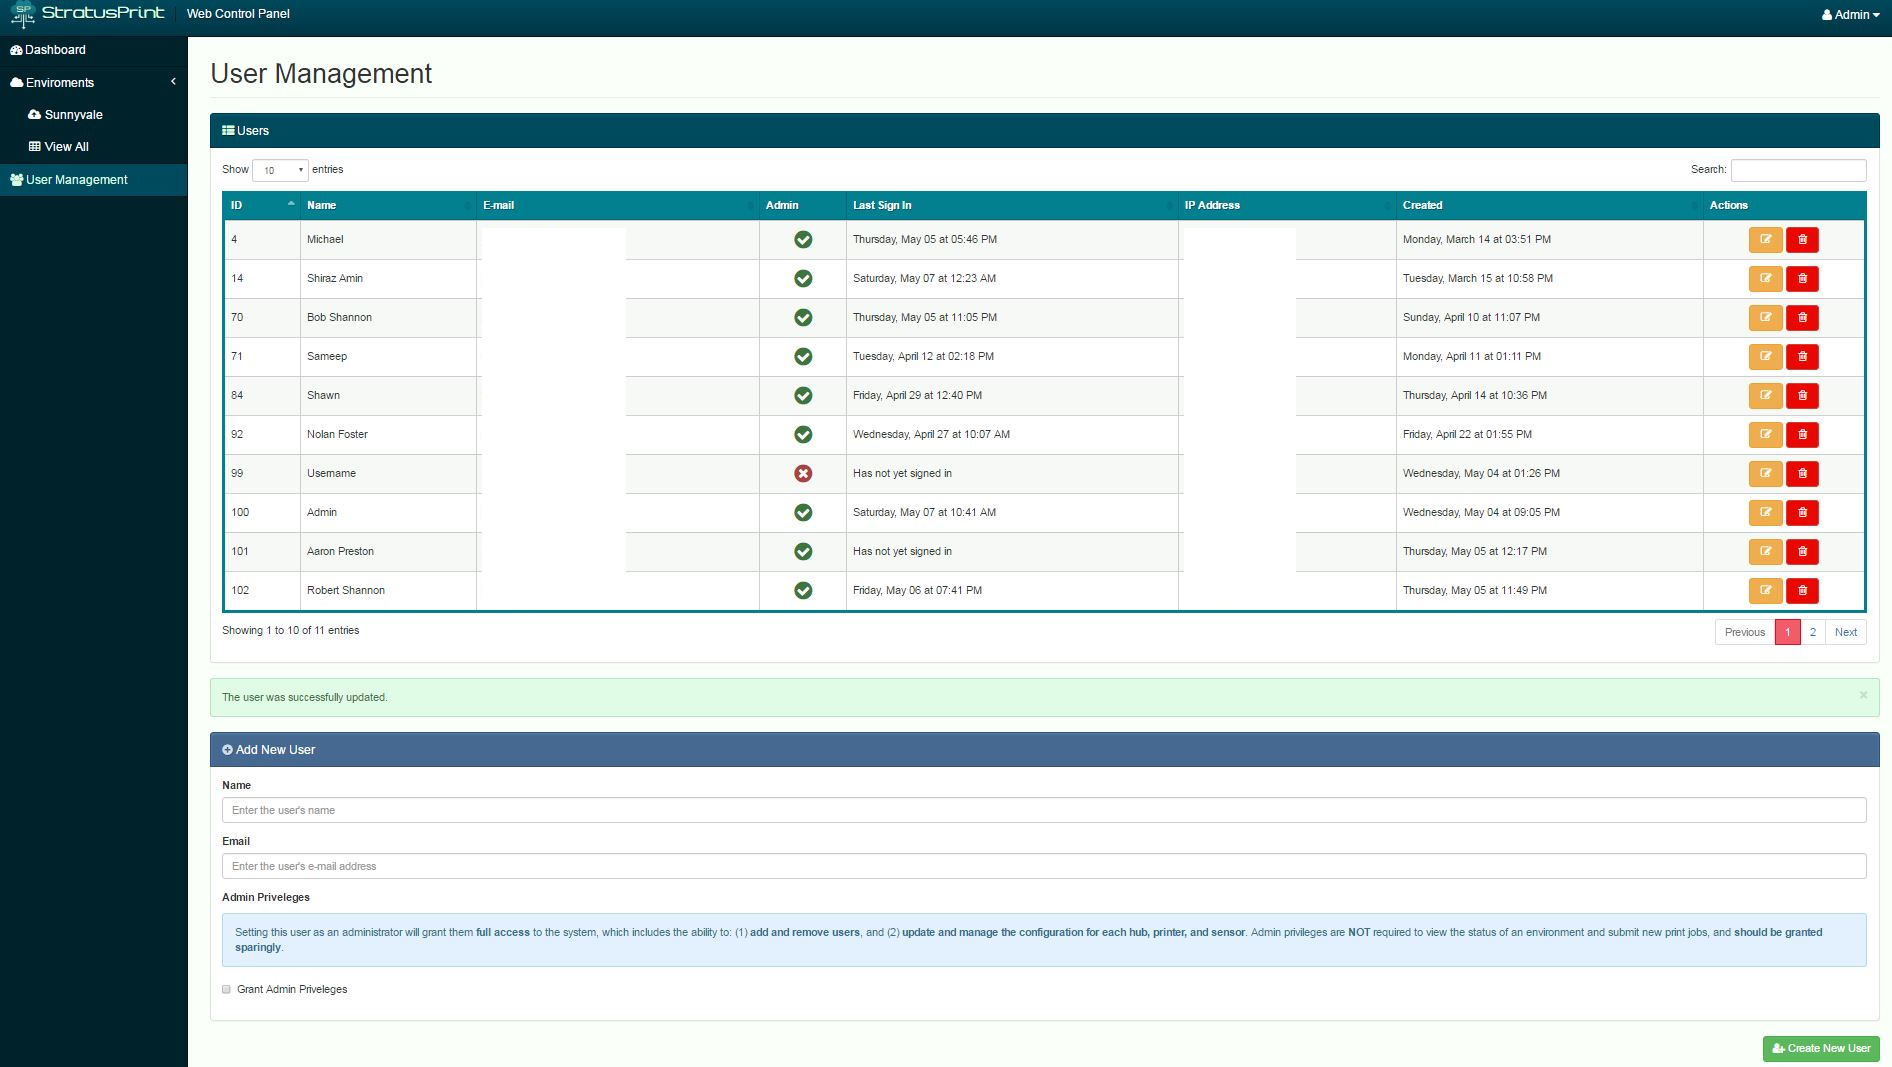
\includegraphics[scale=.15]{images/user-manage.png}
    \end{center}
    \begin{enumerate}
      \item \textbf{Adding a User:} Scroll down to the Add New User portion of the page.  Add the user's name,
      e-mail address, and check the box titled "Grant Admin Privileges" if you would like the user to be an
      admin.  You will receive a confirmation message below the "Users" section if successful.

      \item \textbf{Deleting a User:} Click the red trash icon under the "Actions" column to remove a user.
      You will receive a confirmation message below the "Users" section if successful.
      \begin{center}
        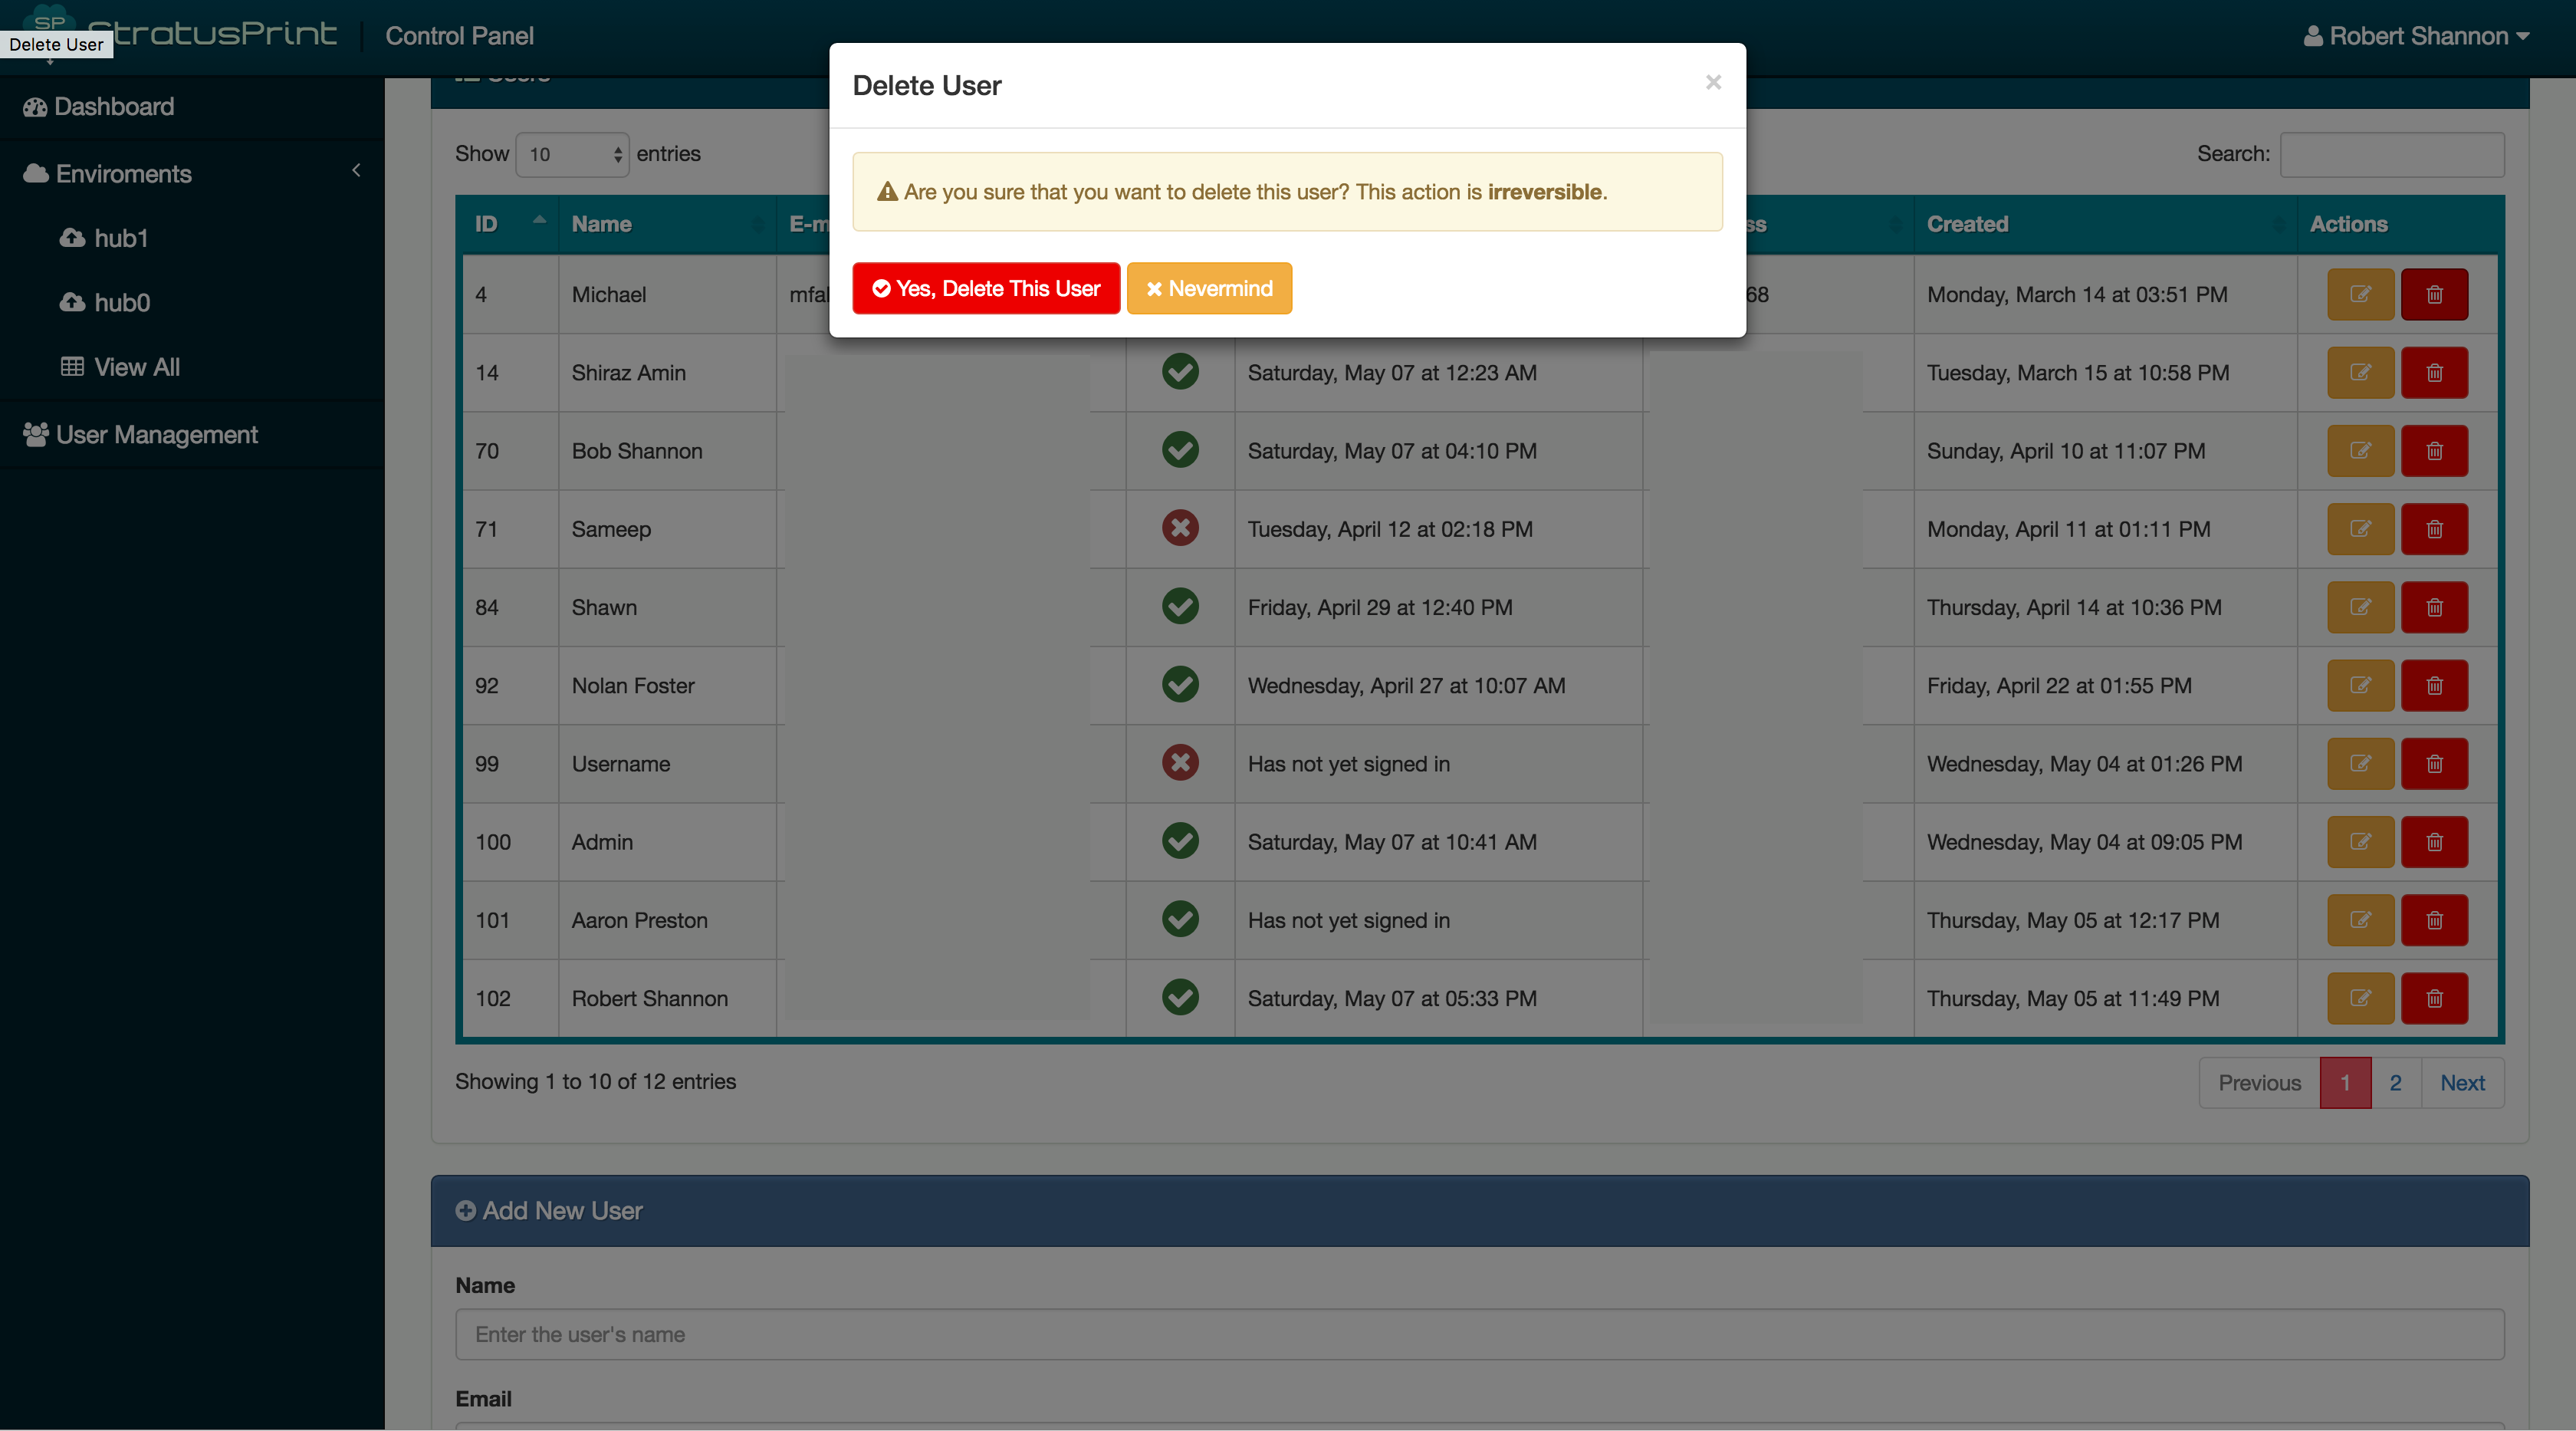
\includegraphics[scale=0.15]{images/delete_user_screenshot.png}
      \end{center}
      \item \textbf{Managing a User:} Click the yellow notepad icon under the "Actions" column to edit user
      details (Name, Email Address, or Add/Remove Admin Privileges).  Then click the "Edit User" button to confirm.
      You will receive a confirmation message below the "Users" section if successful.
      \begin{center}
        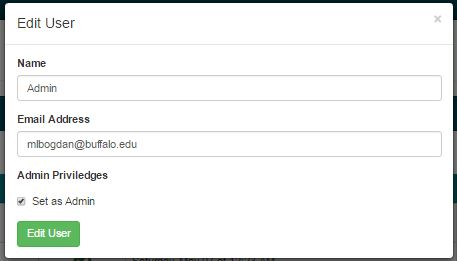
\includegraphics[scale=0.30]{images/user-edit.png}
    \end{center}
    \end{enumerate}

  \subsection{Set up - User}
      Contact your administrator and request a username and password. When they set up your account,
      you will receive an e-mail titled "Confirmation instructions".  Click the link titled \textbf{Confirm
      my account}, then login using the username and password contained in the email.  The password is case-sensitive.
      \begin{center}
      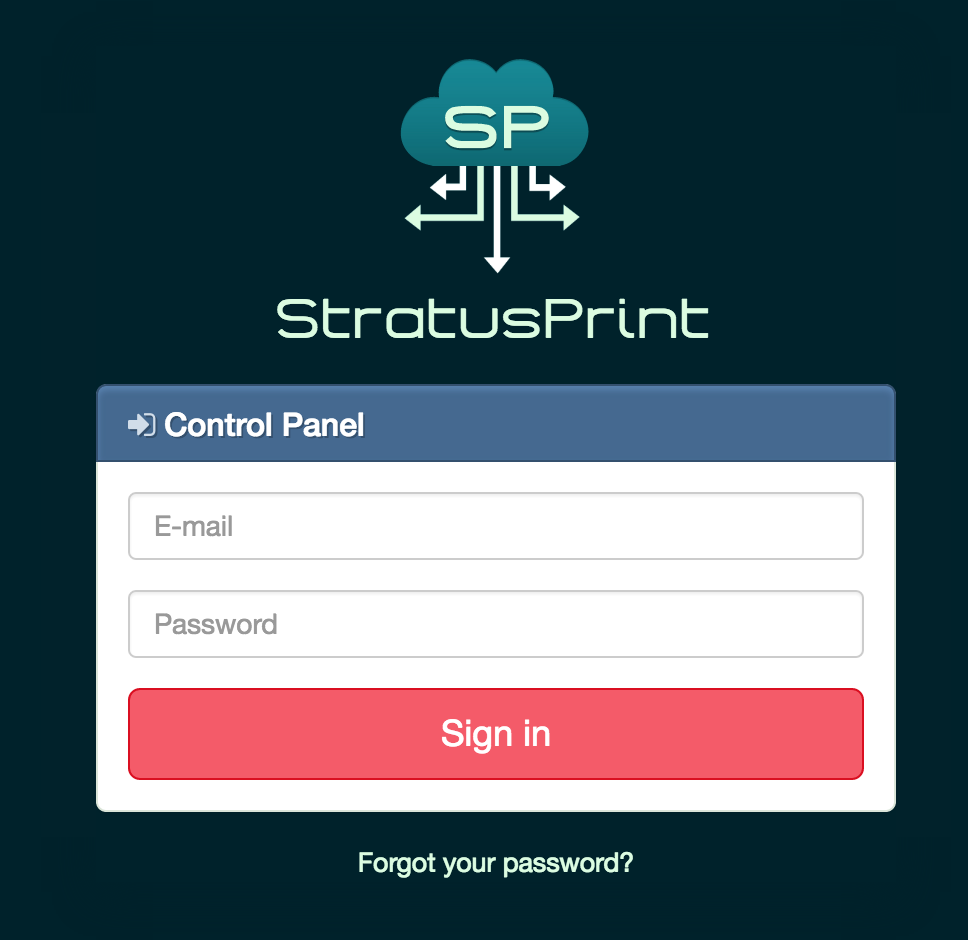
\includegraphics[scale=.5]{images/login.png}
    \end{center}
      Once you have entered your username and password correctly, you will see the dashboard page.

\newpage
  \subsection{Dashboard Page}
      \begin{center}
      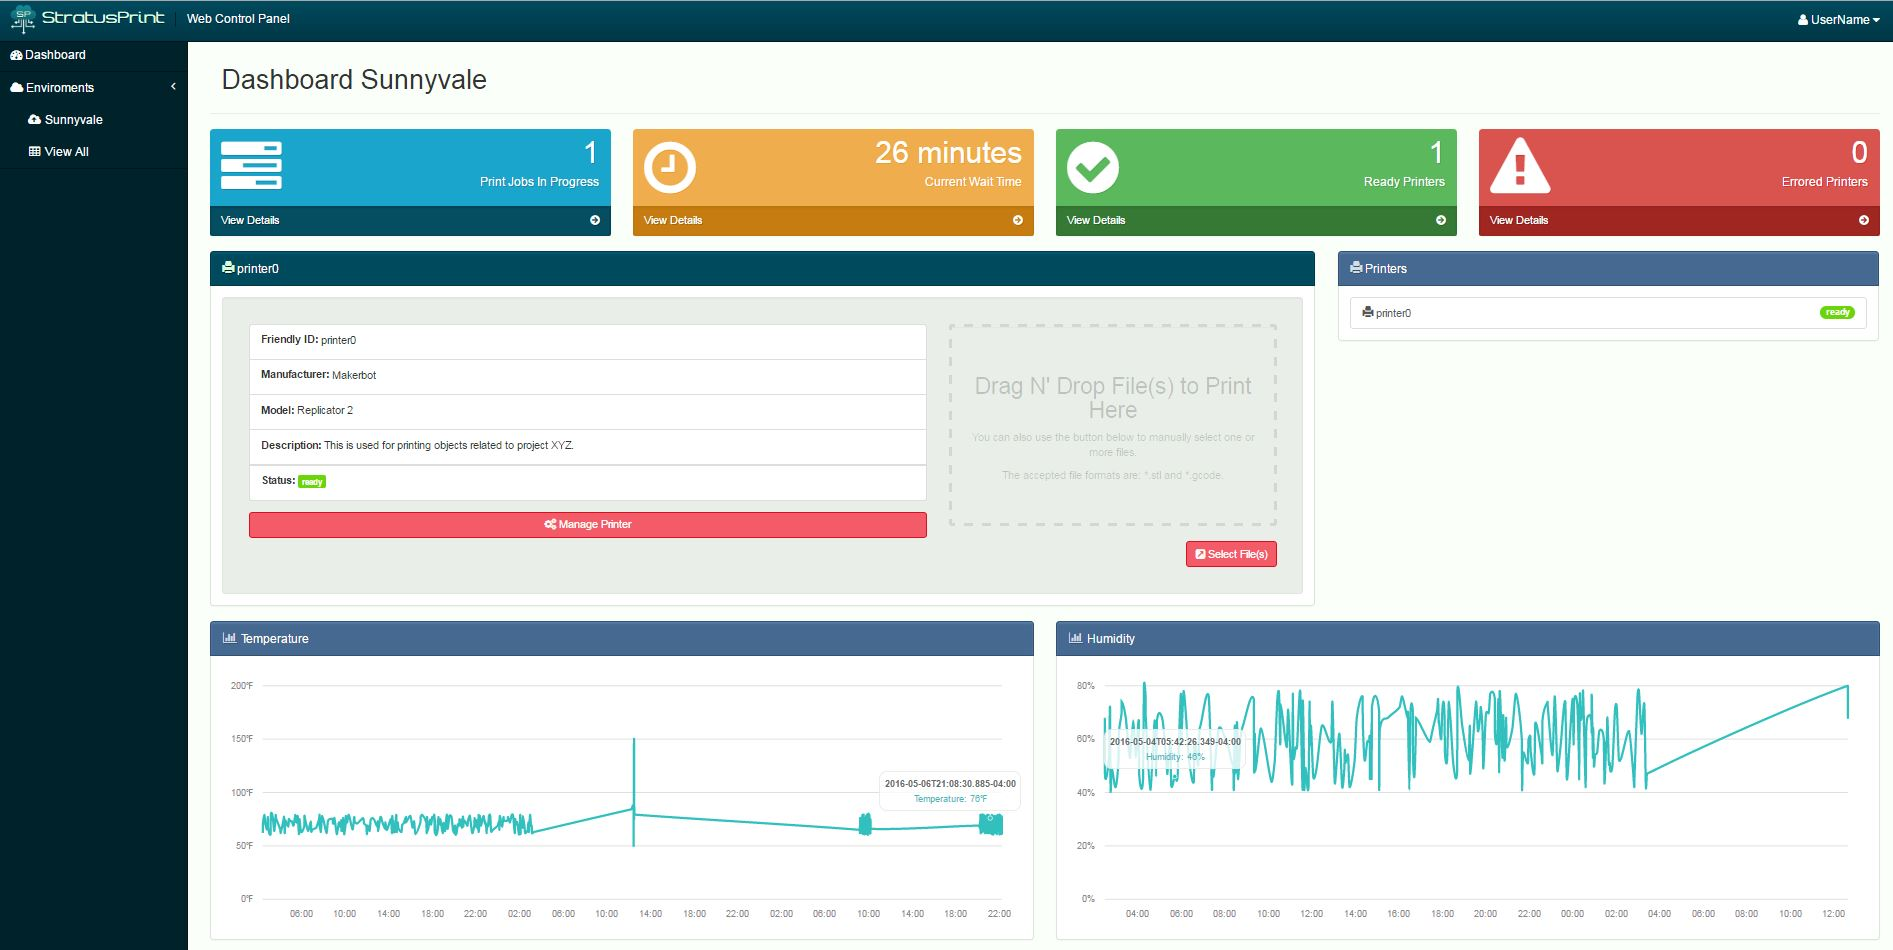
\includegraphics[scale=.15]{images/dash-user.png}
    \end{center}
      The Dashboard Page displays current print job information.\\
      Along the top, you will see print jobs in progress, the wait time until the job is completed, the number
      of printers that are online, and the number of printers with errors.  Click the \textbf{View Details} under
      each option to see more details, including the temperature and humidity of the room, and whether the door
      to the room is open or closed.

  \subsection{Starting a Print Job}
      To upload a file, either drag-and-drop the file into the box labeled \textbf{Drag N' Drop File(s)}, or
      click the \textbf{Select File} button, select the file you would like
      to print, and click the \textbf{open} button.  Your file will be uploaded to the website.  If the file seems to be taking longer than expected to upload, click the \textbf{cancel} button, and try uploading your file again.
      \begin{center}
      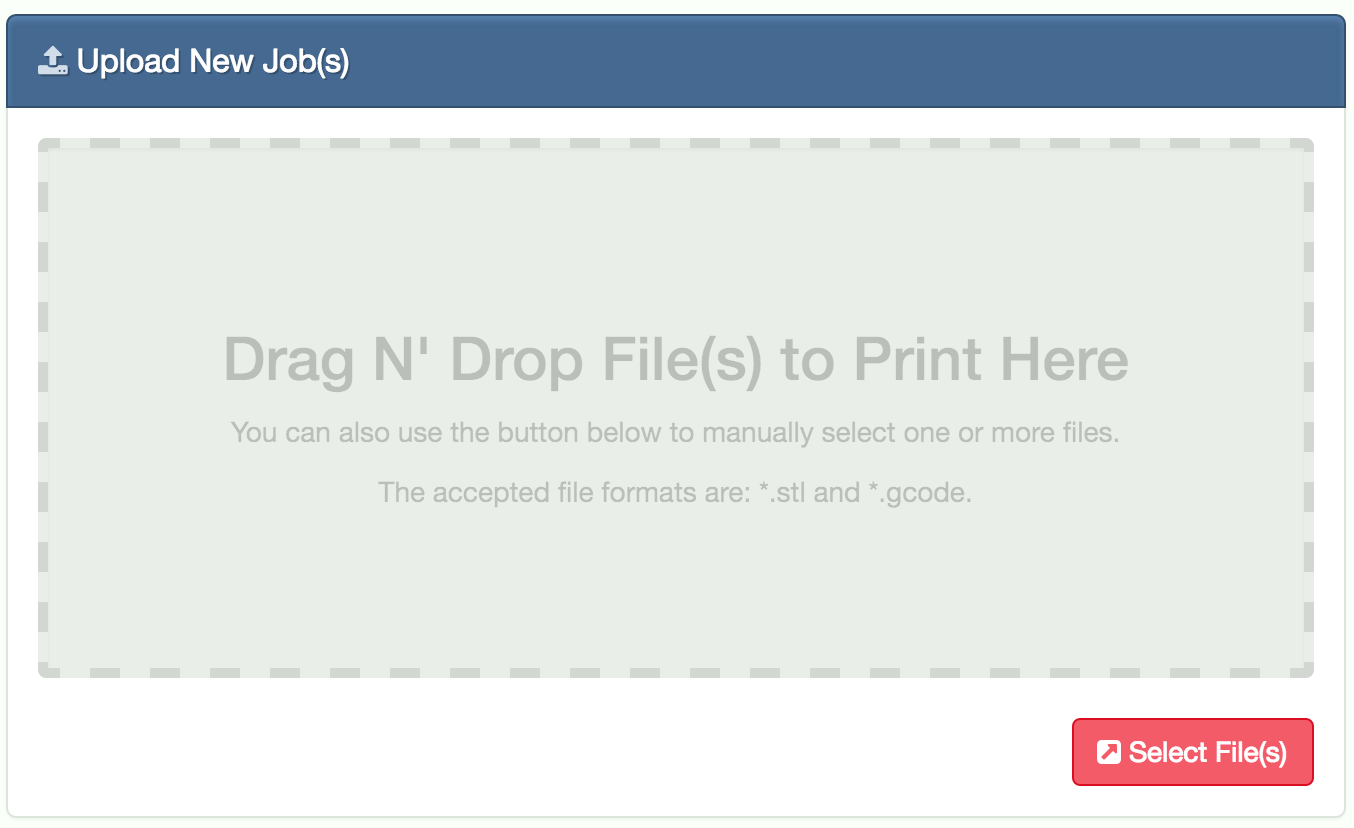
\includegraphics[scale=.25]{images/upload-job.png}
    \end{center}
	Your file will be added to the print queue.  There are two ways to start a print job:\\	
	\textbf{via the Webpage:} If there is no current print job, the \textbf{Start next job} button will be available.  If the print bed is cleaned off, and there are no previously printed objects on the bed, you can click this button to start the next job in the queue.\\
	\textbf{via the Webpage:} If the red light on the control box is blinking, a print job has finished.  Remove the printed object, clean the print bed, then press the button \textbf{ONCE} to start the next job in the queue.  \emph{Wait 20 seconds for the light to stop blinking after pressing the button.  It may take up to 20 seconds for the light to stop blinking while the next job in the queue is being processed!} 
      \begin{center}
      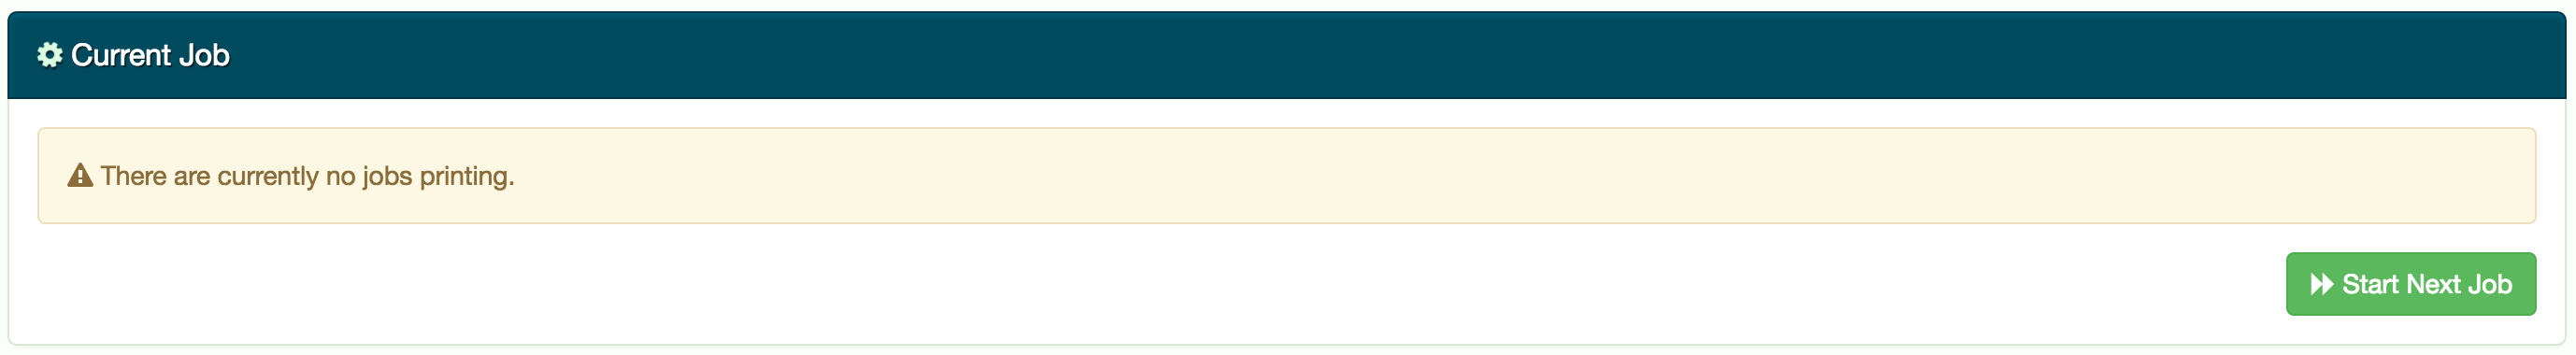
\includegraphics[scale=.3]{images/start-next.png}
    \end{center}


  \subsubsection{Managing Jobs}
      Click the \textbf{Manage Printer} button at the bottom of the page.  You will see information about the job in progress.\\
      To start, pause, and cancel a job, click the corresponding buttons. 
      \begin{center}
      
\includegraphics[scale=.8]{images/job-buttons.png}
    \end{center}
You can see previously issued commands in the bottom right of the screen.
      \begin{center}
      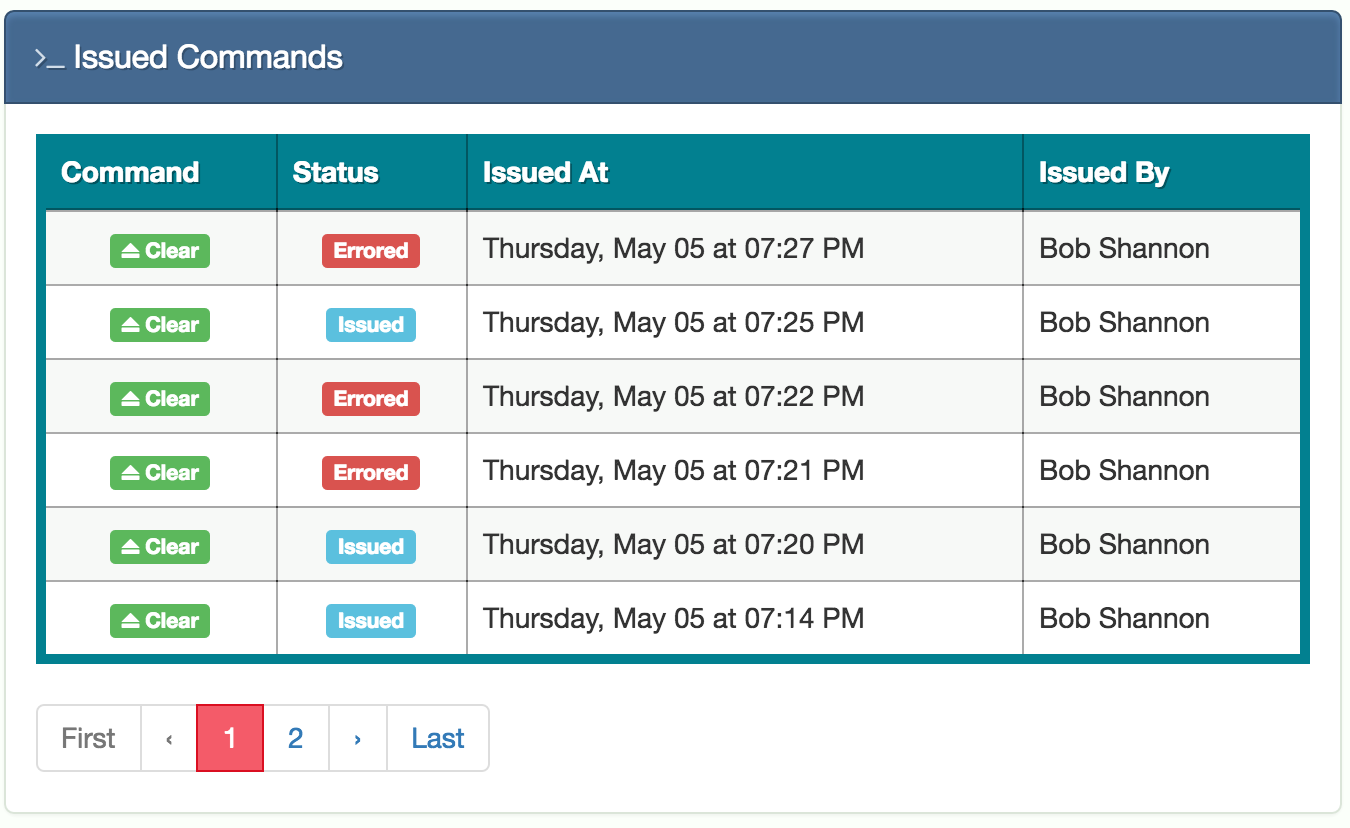
\includegraphics[scale=.3]{images/issued-commands.png}
    \end{center}

  \subsubsection{Managing Printers, Adding Sensors, or other Admin Tasks}
      Consult the provided technical documentation for information on how to perform advanced tasks.

